
\section{Societal Impacts}
\label{sec:social impace}
\nj{Our paper is closely related to Responsible AI (RAI), especially in enabling qualitative assessments of models. Our approach provides visual and intuitive explanations of a model’s decision-making criteria, offering insights that are both explanatory and responsible. Our approach of utilizing DSVs for RAI enables global explanations, surpassing traditional Explainable AI (XAI) methodologies, which usually focus on local explanations for individual inputs and cannot provide a global decision criterion. % as opposed to our DSVs. 
Furthermore, since our method is based on model inversion, it ensures safety and privacy.
While the synthesized sets in Fig.~\ref{fig:DSVSET} might appear similar to the selected sets, they do not replicate specific sample features. This is because DSVs represent a more generalized decision boundary, avoiding the inclusion of image-specific features. Consequently, DSVs enable all models using logistic loss to be more responsible.}

%\jh{Our paper is closely related to Responsible AI (RAI), particularly in terms of enabling qualitative assessment of models. They provide a visual and intuitive explanation of a model's decision-making criteria, offering insights into how the model operates that are not only explanatory but also responsible. This approach goes beyond traditional Explainable AI (XAI) methodologies, which typically focus on local explanations for individual inputs and lack the ability to offer a global decision criterion like DSVs. Additionally, as this method is based on model inversion, it ensures safety and privacy. Although the synthesized sets in Fig.~\ref{fig:DSVSET} might look similar to the selected sets, they do not replicate specific sample features. This is because DSVs represent a more generalized decision boundary, thus avoiding the inclusion of image-specific features. Therefore, DSVs can make all models using logistic loss responsible.}

\begin{figure}[h]
  \centering
   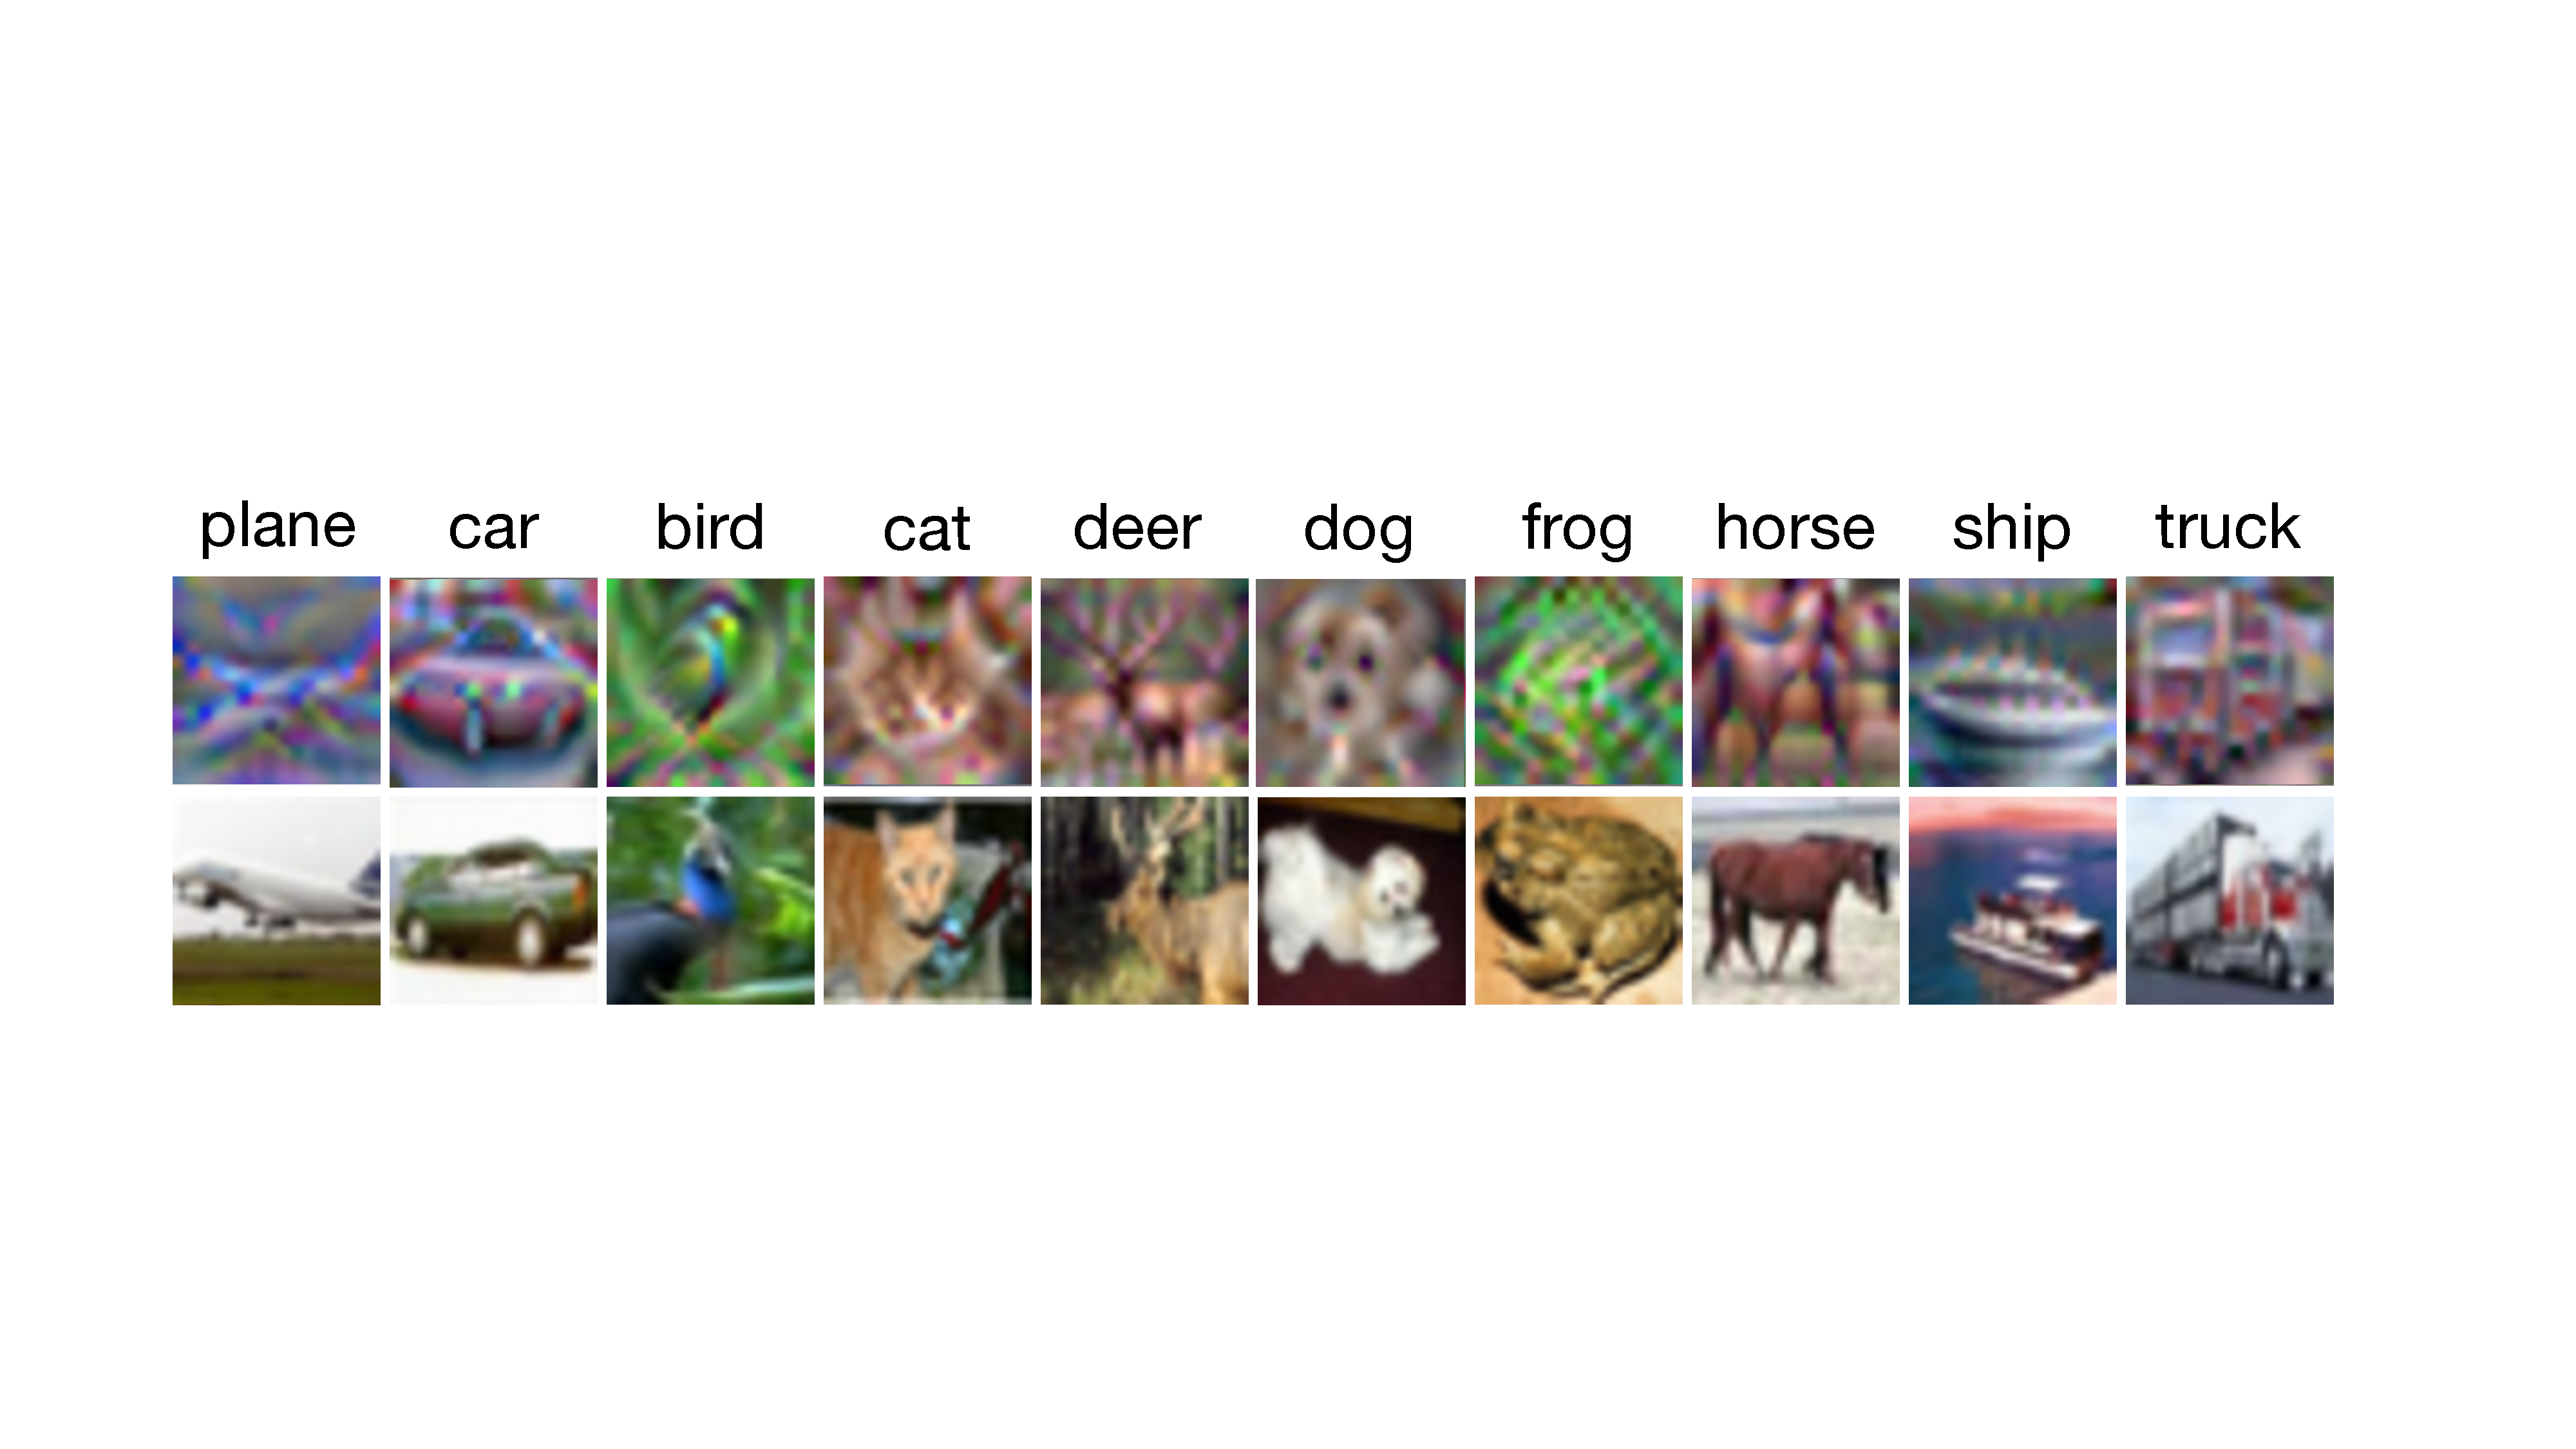
\includegraphics[width=1.0\linewidth]{./figure/dsvset.pdf}
   % \includegraphics[width=0.8\linewidth]{author-kit-CVPR2024-v2/figure/manifoldfigure.pdf}
   \caption{Comparison of synthesized images (first row) created using the DeepKKT condition initiated from noise, and selected images (second row) from the CIFAR-10 training dataset. The selected images were chosen based on \nj{$\lambda$} values, \nj{\ie each image has} the highest \nj{$\lambda$} in each class. Both synthesized and selected images demonstrate similarity at the pixel level sharing common features.}
   \label{fig:DSVSET}
\end{figure}

\section{Limitations and Future work}

\label{sec:limitations}

\nj{In this paper, we propose the DeepKKT condition, which can be applied universally to any deep models to generate deep support vectors (DSVs) that function similarly to support vectors in SVMs.} 
%In this paper, we propose the DeepKKT condition, which can be applied unconditionally to \nj{any} deep models, \nj{to generate} deep support vectors (DSVs) that function similarly to support vectors in SVMs. 
However, \nj{it should be noted that} the equivalence \nj{between DSVs in deep learning models and support vectors in SVMs is only described intuitively, not rigorously.} % and the rigorous proof that the DeepKKT condition must be as we proposed \nj{are} different. 
We have shown experimentally \nj{in Fig.~}\ref{fig:DSVSET} and intuitively \nj{in Sec.~}\ref{sec:overparam} why the DeepKKT condition should be as we suggested, but we have not derived it \nj{with rigorous math.} %mathematically rigorously.
Proving this rigorously %theoretically 
would be a meaningful research \nj{topic}.



\section{Intutive explanation of DeepKKT condition}
\label{sec:overparam}

\begin{figure}[t]
  \centering
   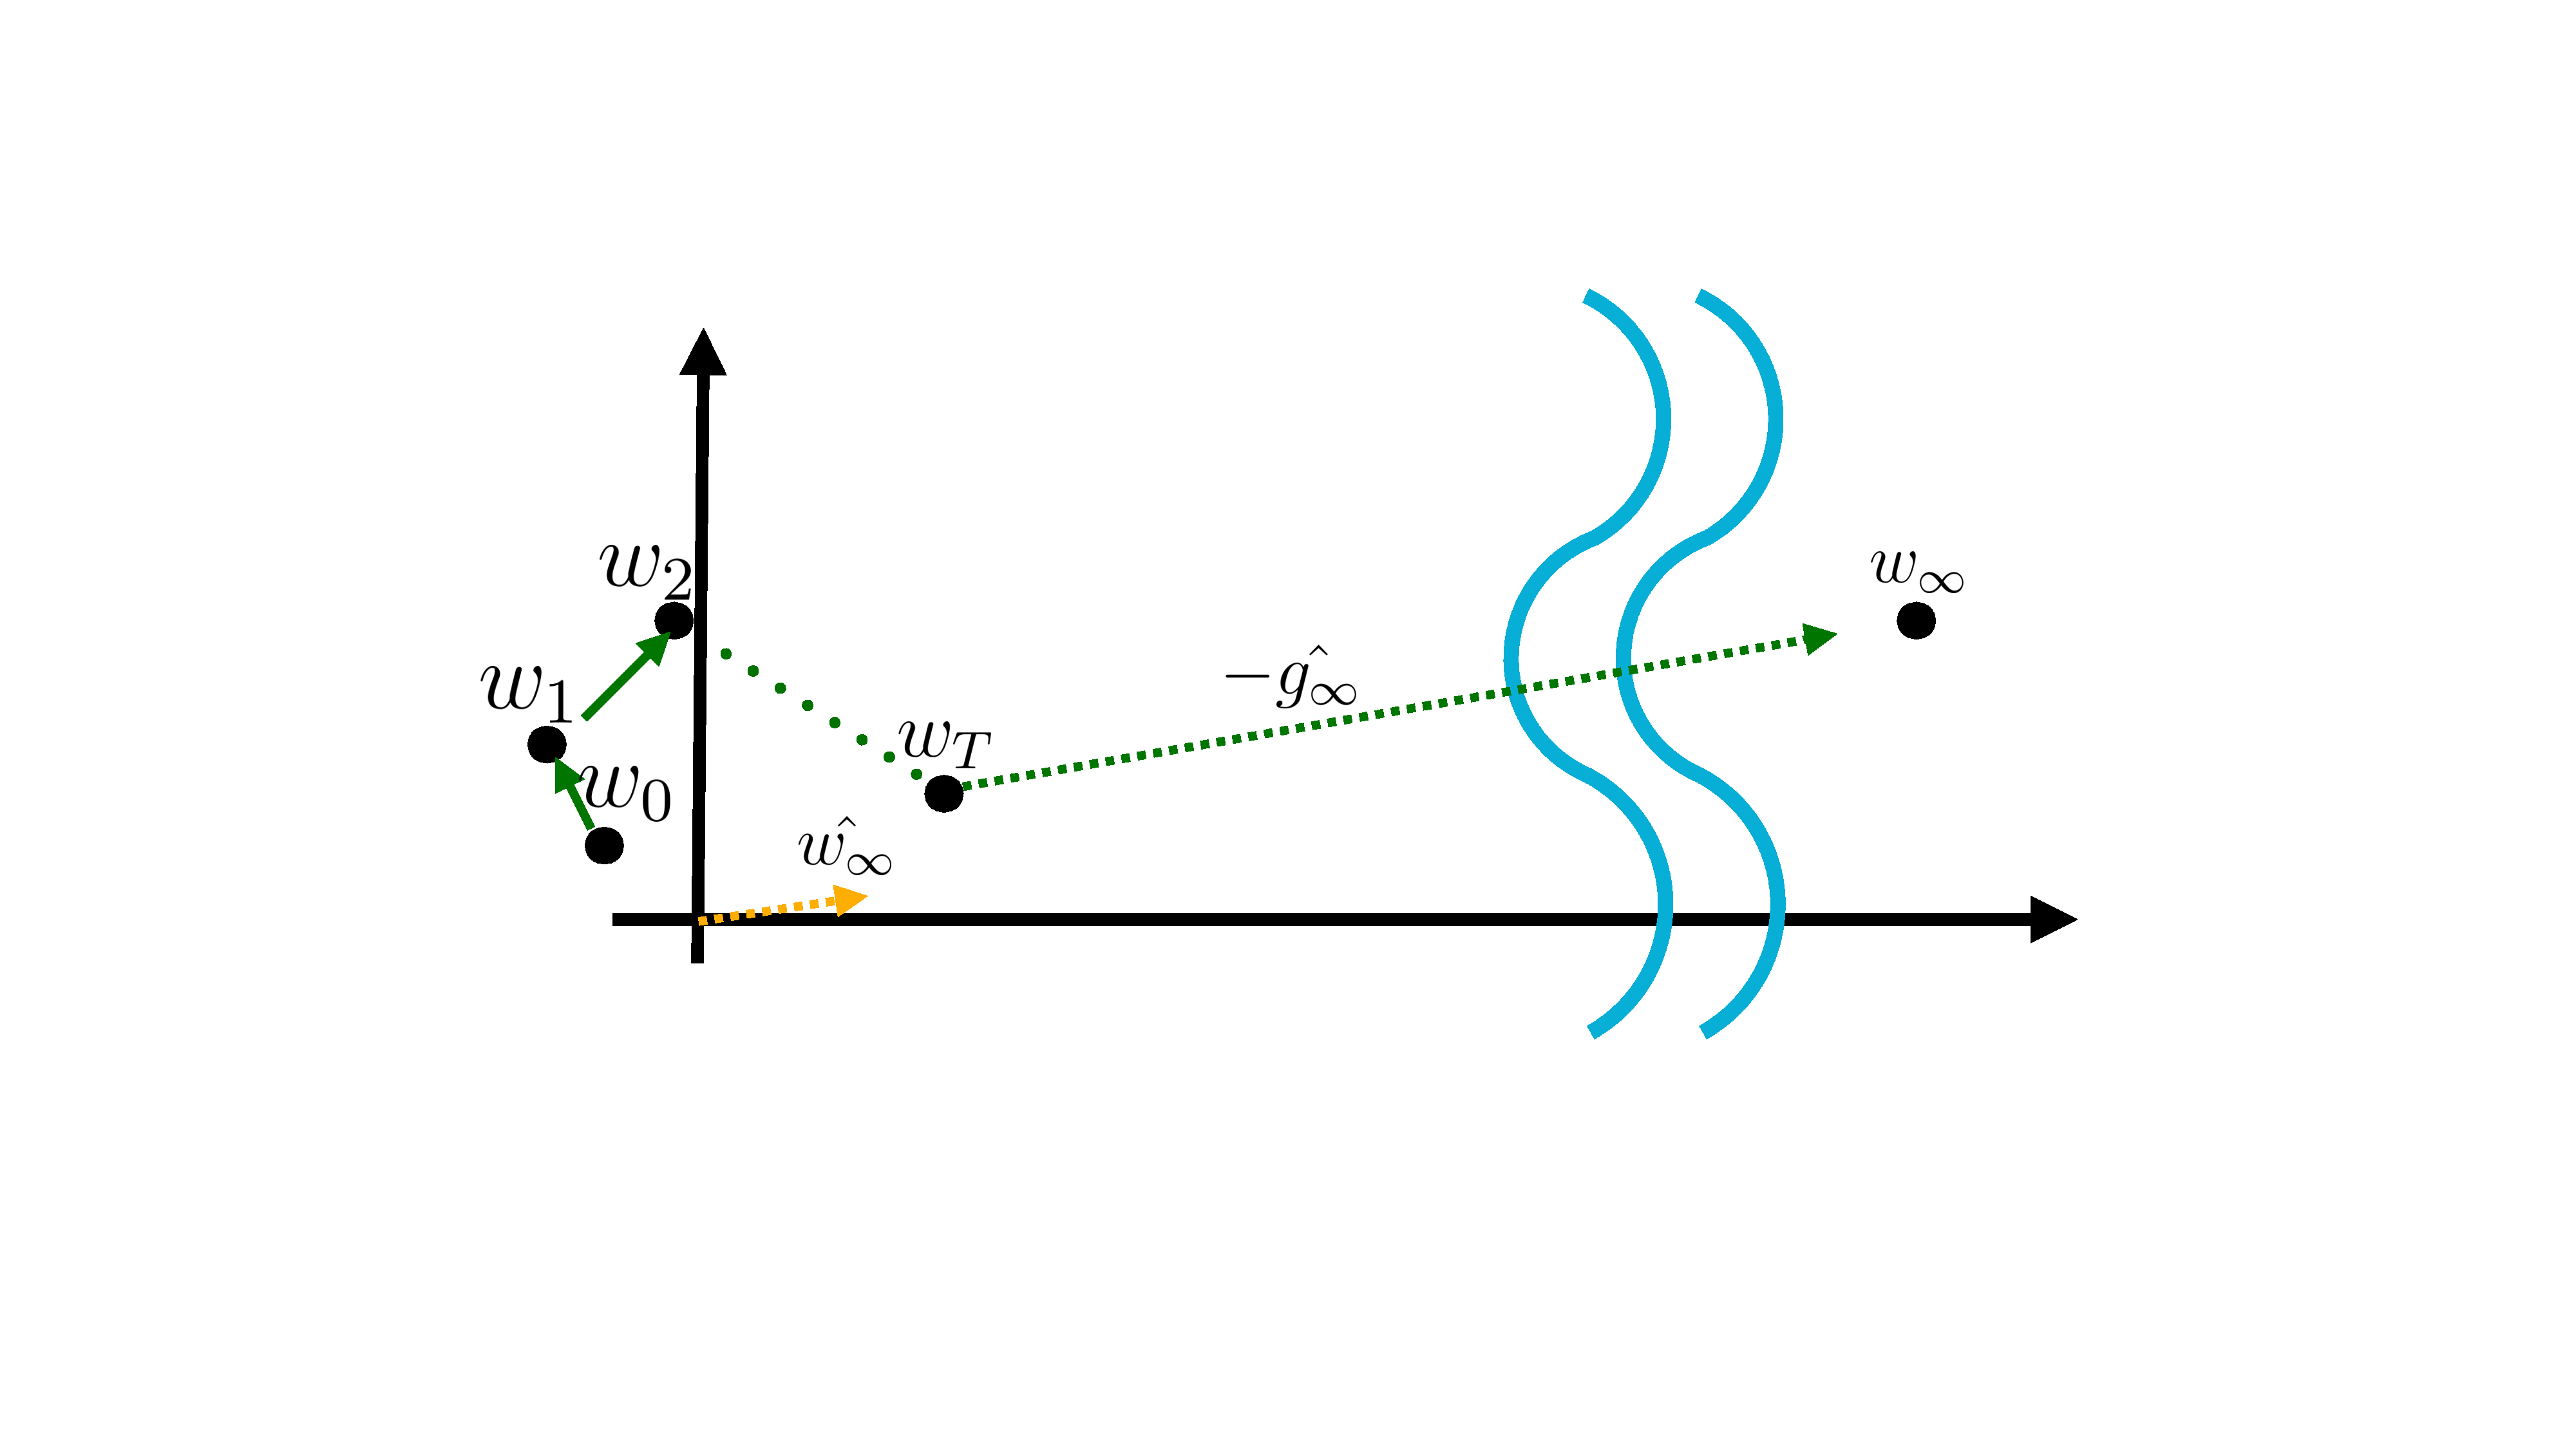
\includegraphics[width=0.9\linewidth]{./figure/intuitive.pdf}
   \caption{\jh{The stationarity condition with a logistic loss. Even though the direction of the gradient $\hat{g}$ converges, the size of the gradient does not go to zero. Therefore, the direction of the converged gradient weight $\hat{w_\infty}$ aligns with $\hat{g}$.}}
   % \caption{\jh{An intuitive explanation on stationarity conditions. When we use logistic loss, even the direction of gradient $\hat{g}$ converges, the size of gradient does goes to zero. Therefore, the converged gradient weight's direction $\hat{w}$ follows $\hat{g}$}}
   \label{fig:intuitiveun}
\end{figure}


%\jh{In DeepKKT, \nj{all the conditions, except one make} sense. For example, \nj{the} primal \nj{feasibility} condition and \nj{the} manifold condition \nj{make} sense and dual condition can be regraded as importance sampling. The most counterintuitive part is stationarity section.}
\nj{In DeepKKT, many conditions make sense, except for one. For instance, the primal feasibility condition and the manifold condition are reasonable, and the dual feasibility condition can be regarded as importance sampling. However, the most counterintuitive part is the stationarity condition:}
%
\begin{equation}
\hh{L_{\text{stat}} = D(\theta^*, -\sum_{i=1}^n \lambda_i \nabla_\theta L(\Phi(x_i;\theta^*), y_i))}
\end{equation}

%\jh{In this \nj{part, we are} to explain the dynamics of overparameterized deep learning, and explain how it is connected to deep learning. Below is an analogy of \cite{svm:theory}.}
\nj{In this section, we will explain the dynamics of DSVs in an overparameterized deep network and how it is connected to deep learning. Below is a quick analogy of \cite{svm:theory} to illustrate this connection.}

A deep learning \nj{model} follows \nj{the} following ODE:

\begin{equation}
    w_{t+1} = w_t - \eta \nabla L(x,y;w_t).
\end{equation}

% \jh{Where $\alpha$ is learning rate and $t$ is optimization step. $L$ does not goes to zero since deep learning model ususally exploits a function with logitic tail such as cross entropy function. So there exists an convergece of gradient direction $g_\infty \defeq \hat{\nabla L}$. And there exists $T$ where the gradient direction converges to $g_\infty - \varepsilon$ For sufficient small $\varepsilon$. Then, as illustrated in Fig.~\ref{fig:intuitiveun}, $w$ moves toward the direction of $-g^\infty$, Therefore $\hat{w_\infty} \simeq -g_\infty$ }

\jh{\nj{Here,} $\eta$ is the learning rate and $t$ is the optimization step. \nj{The loss} $L$ does not go to zero since deep learning models usually exploit a \nj{loss} function with a logistic tail, such as the cross-entropy \nj{loss}, and the gradient of the least confident sample (support vector) dominates overall gradient. Thus, there exists a convergence of the gradient direction $g_\infty \coloneqq \hat{\nabla} L$. There also exists a time $T$ where the gradient direction converges to $g_\infty - \varepsilon$ for a sufficiently small $\varepsilon$. As illustrated in Fig.~\ref{fig:intuitiveun}, $w$ moves toward the direction of $-g_\infty$. Therefore, $\hat{w}_\infty \approx -g_\infty$.}

\jh{This is \nj{for what} stationarity condition wants to seek. The direction of $g_\infty$, by using only \nj{a} few support vectors.}

\section{Implementation Details}
\label{sec:detail}

 %To obtain the pretrained weight $\theta^*$, 
To obtain the results in Table~\ref{table:fewshot} and Fig.~\ref{fig:transfer}, the ConvNet architecture~\cite{convnet} was used for pretraining \(\Phi(\cdot; \theta)\) on the \nj{SVHN} dataset~\cite{dataset:svhn},} a digit dataset with dimensions similar to CIFAR-10~\cite{dataset:cifar10}. \jh{For ImageNet, we used \nj{the} ResNet50 model~\cite{resnet} with \nj{the} original setting \nj{in the paper}. Specifically, we used \nj{the} pretrained model in torchvision library in pytorch~\cite{pytorch}. \jh{For visualizing synthesized DSVs in ImageNet, we increased the contrast in 224x224 dimensions.} When calculating $L_\text{stat}$, we averaged the distance per parameter. \nj{In Alg.~\ref{alg:KKT}, $\eta$ was set to 5.}}


\jh{To synthesize DSVs in ImageNet, we used translation, crop, cutout, flip, and noise for augmentation, with hyperparameters set to 0.125, 0.2, 0.15, 0.5, and 0.01, respectively. In Eq.~(\ref{eq:main_equation}), we set $\alpha$ to 2e-5, $\beta$ to 40, and $\gamma$ to 1e-6. When calculating $L_\text{stationarity}$, we averaged the distance per parameter.}

\jh{For dataset distillation in Table~\ref{table:fewshot}, we used translation, crop, flip, and noise for augmentation, with hyperparameters set to 0.125, 0.2, and 0.5, respectively. In Eq.~(\ref{eq:main_equation}), we set $\alpha$ to 2e-3, and both $\beta$ and $\gamma$ to 0. For retraining models with synthesized images, we used a learning rate of 1e-4 while \nj{the other parameters set to the default values of} the Adam optimizer~\cite{ADAM}.}


% {\nj{To synthesize} %retraining the model with 
% DSVs, In imagenet, we used translation, crop, cutout, flip, noise for augmentation and the hyperparameter is 0.125, 0.2, 0.15, 0.5, 0.01, respectively. In eq.~\ref{eq:main_equation}, we set $alpha$ for 2e-5, $\beta$ for 40, $\gamma$ for 1e-6. In calculationg $L_\text{stationarity}$ we averaged the distance per parameters,
% the
% large learning rate of 0.1 and a $\rho$ value of 0.0001 were utilized for the SAM optimizer to adhere to the principle of margin maximization~\cite{ADAMj
% For \(L_\text{stat}\), we set $\alpha_x = 10^{-3}$, $\alpha_\lambda = 0.1$, and $\gamma = 5$, respectively.

% \jh{For dataset distillation, we used learning rate 0.0001 for re-training models through distilled images in Adam\cite{adam} optimizer. Other parameters are set default. }
% \jh{For synthesis, it took 15 minutes in a single 1080TI GPU in CIFAR10. We leave additional details in Appendix Sec.\ref{appendix:details}}
% \label{appendix:details}
% \jh{For \(L_\text{stat}\), we set $\alpha_x = 10^{-3}$, $\alpha_\lambda = 0.1$, and $\gamma = 5$, respectively. This was due to the differing scales. The actual computed loss for stationarity was ten times higher than for primal loss. }
%To satisfy the manifold condition in reconstructing DSVs, we implemented techniques from the \nj{diffusion model}~\cite{diffusion:latent1}. This involved synthesizing data at a low resolution, then upscaling it to a higher resolution. We initially downscaled the image twice, then upscaled it, continuing with optimization. 
% To reduce the impact of outliers, we choose the $L_1$ metric and apply the square root to \hh{the gradient term} when measuring distance.}

\nj{To obtain the pretrained weight $\theta^*$ for CIFAR10 and CIFAR100,} we chose the ConvNet architecture~\cite{convnet}, a common choice in deep learning. This architecture includes sequential convolutional layers followed by max pooling, and a single fully-connected layer for classification. The learning rate was set to \nj{\(10^{-3}\)} with a weight decay of \nj{\(0.005\)} using the Adam optimizer. Additionally, we employed flipping and cropping techniques, with settings differing from those used for DSVs reconstruction to ensure fair comparison. For pretraining \(\Phi\) on the Street View House Numbers (SVHN) dataset~\cite{dataset:svhn}, a digit dataset with dimensions similar to CIFAR-10~\cite{dataset:cifar10}, we exclusively trained the fully-connected layer of the CIFAR-10 pre-trained ConvNet. This approach resulted in a training accuracy of 80\%. 
% \jh{When retraining the model with DSVs, we used large learning rate of 0.1 and a $\rho$ value of 0.0001 were utilized for the SAM optimizer to adhere to the principle of margin maximization~\cite{largelr, samopt}.}
% \jh{For DSVs synthesis, we used a single 1080TI GPU and it took 15 minutes.}
% \section{Conventional methods rely on training dataset}

% \label{sec:reliance}
% % Please add the following required packages to your document preamble:
% % \usepackage{multirow}
% \begin{table}[]
% \centering
% \caption{Dropping Accuracy in gradient matching}
% \begin{tabular}{|c|c|c|}
% \hline
% img/cls            & data rate & Dataset Condensation \\ \hline
% \multirow{3}{*}{1} 
%                    & 10\%      & 37.9  $\pm$ 0.76     \\
%                    & 5\%       & 33.6$\pm$ 1.42       \\
%                    & 1\%       & 27.8$\pm$ 0.65       \\ \hline
% \end{tabular}
% \end{table}

% \jh{Table.~\ref{table:dropacc} shows that current dataset distillation techniques heavily relies on the size of gradient. In talbe, we constraint the size of accessible datasets in gradient matching. And the results show that the performance drops as we reduce the size of training dataset.}
% \section{Catalog of DSVs}
% \label{sec:catalog}
% \subsection{Dataset Condensation}

% Our algorithm fundamentally defines and seeks deep support vectors (DSVs), which are the backbone of the model. \hh{Considering} that the number of DSVs is substantially smaller than the entire dataset, our approach can naturally be considered a dataset distillation problem. \cite{}

% The primary goal of dataset distillation is to enhance privacy and reduce communication load by creating a smaller dataset that retains equivalent performance to the original dataset \hh{via} gradient matching\cite{}. It involves using the original dataset to generate hundreds of models\cite{}, or in other words, to minimize the gradient difference when the original data \( x \) and the distilled data \( \tilde{x} \) are fed forward through the trained model \( \theta \). This process necessitates high computational cost due to the use of the entire dataset and even requires the Hessian when trajectory matching is performed \cite{}. Those requirements imply that conventional dataset distillation algorithm should be performed in central node which can process high-order computation and memory cost algorithm. \hh{However the process of centralizing data processing creates a challenging situation, as the data comes from edge devices like smartphones. Moving raw data from these devices to a central system ends up causing the privacy and communication issues that dataset distillation is supposed to solve. Therefore, the solution to dataset distillation needs to happen on the edge devices, without the need to send out the training data.} 

% \hh{이텔릭이나 headings로 조건들 나열하기}
% However, storing the entire dataset at the edge is impractical due to the significant computational burden involved in gradient matching. Moreover, the continuous learning setting, often presupposed at the edge, cannot be accommodated due to these constraints. Holding data for gradient matching introduces privacy risks, akin to those in other generative models, and these are not fully alleviated even when datasets are synthesized using GANs trained with the original dataset.

% In contrast, our DSV methodology inherently overcomes these issues. \hh{Our algorithm, which does not require any access to training data, could provide a viable solution to privacy concerns. Moreover, the computational cost of this approach is on par with that of initial model training. In the perspective of the resolution on DSVs, results[?] indicate a significant advantage in that our method can achieve comparable performance even with low-resolution DSVs. Furthermore, this approach allows for a flexible trade-off depending on computational resources: lower resolution DSVs can be employed in scenarios with limited computational capacity, while higher resolution DSVs can be utilized in edge devices with more computational leeway. This flexibility in managing the trade-off between DSV resolution and computational demand constitutes a key strength of our methodology.} 

% \subsection{Global Explanation}
% DSVs offer a unique advantage in the realm of Explainable AI (XAI) by providing a mechanism for extracting support vectors directly from the model without the need for input data. Considering that support vectors encode the coordinates of the hyperplane, they inherently offer a form of global explanation for each class within natural XAI frameworks. Although the ultimate goal in XAI is to achieve global explanations, the current state of the art predominantly enables only local explanations, which interpret the response of a model \( \theta \) to a given input \( x \). Our algorithm stands out by facilitating global explanations, which is a significant stride in the field of XAI.

% \subsection{Adversarial Attack, Adversarial Training}
% \hh{ In adversarial attacks, the objective is to perturb the model by adding noise of minimal epsilon magnitude. This strategy often exploits the fact that misclassifications commonly occur near the decision boundary, allowing for the effective creation of adversarial examples using Deep Support Vectors (DSVs) close to this boundary. As depicted in Fig.~\ref{fig:adversarial}, even a minimum addition to an image labeled 'dog'—merely 1\% of the size of the 'dog' image—can lead to its misclassification by the model. \jh{This is mainly due to its information-dense-feture of DSVs. DSVs matches the purpose of adversarial attack when used as global adversarial patch.}
% %When crafting adversarial examples, it's crucial to minimally alter the original image while navigating the semantic space. DSVs, possessing high-quality semantic information in the decision boundary space, enable slight modifications without significant distortion of the original image, effectively disrupting the model. \\ 
% \jh{This feature naturally helps adversarial training, a methodology to counteract adversarial attacks.} \jh{This embodies training procedure, where training with a diverse range of augmented images} However, there typically exists a trade-off between generalized clean accuracy and robust accuracy; i.e. training with various augmentations might enhance robustness but detrimentally affect clean accuracy (proper evaluation of original images). Therefore, efficient augmentation is necessary. Leveraging the insight that adversarial examples are primarily generated near the decision boundary, the extracted DSVs can be simply combined for augmentation in training. The method of extracting DSVs is not only computationally light but also efficient and straightforward in its augmentation approach, making it potentially effective against general adversarial attacks.}



% \begin{table}[]
% \centering
% \caption{Dropping Accuracy in gradient matching}
% \label{table:dropacc}
% \begin{tabular}{c|c|c}
% img/cls & data rate & Dataset Condensation \\ \hline
%      10  & 10\%      &     \\
%         & 5\%       &        \\
%         & 1\%       &       
% \end{tabular}
% \end{table}


\section{DSVs \nj{by} Selection}
% \jh{Fig~\ref{fig:entropyhigh} shows the selected images which has large lagrangian variable $\lambda$, Which correspondes to candidtates used in Fig~\ref{fig:correlation}. Surprisingly, there exists a meaningful match between selected DSVs and synthetized DSVs in CIFAR10 Datasets in Fig~\ref{fig:DSVSET}. It implies that, as synthetizing DSVs corresponds to reconstruct training data which lie in boundary manifolds. }
\jh{Fig.~\ref{fig:entropyhigh} shows the selected images with large Lagrangian multipliers $\lambda$'s, which correspond to the candidates used in Fig.~\ref{fig:correlation}. Surprisingly, there is a meaningful match between the selected DSVs and the synthesized DSVs in the CIFAR-10 dataset, as shown in Fig.~\ref{fig:DSVSET}. This implies that synthesizing DSVs corresponds to \nj{reviving} training data that lie on the boundary manifolds.
}
\begin{figure}[h]
  \centering
   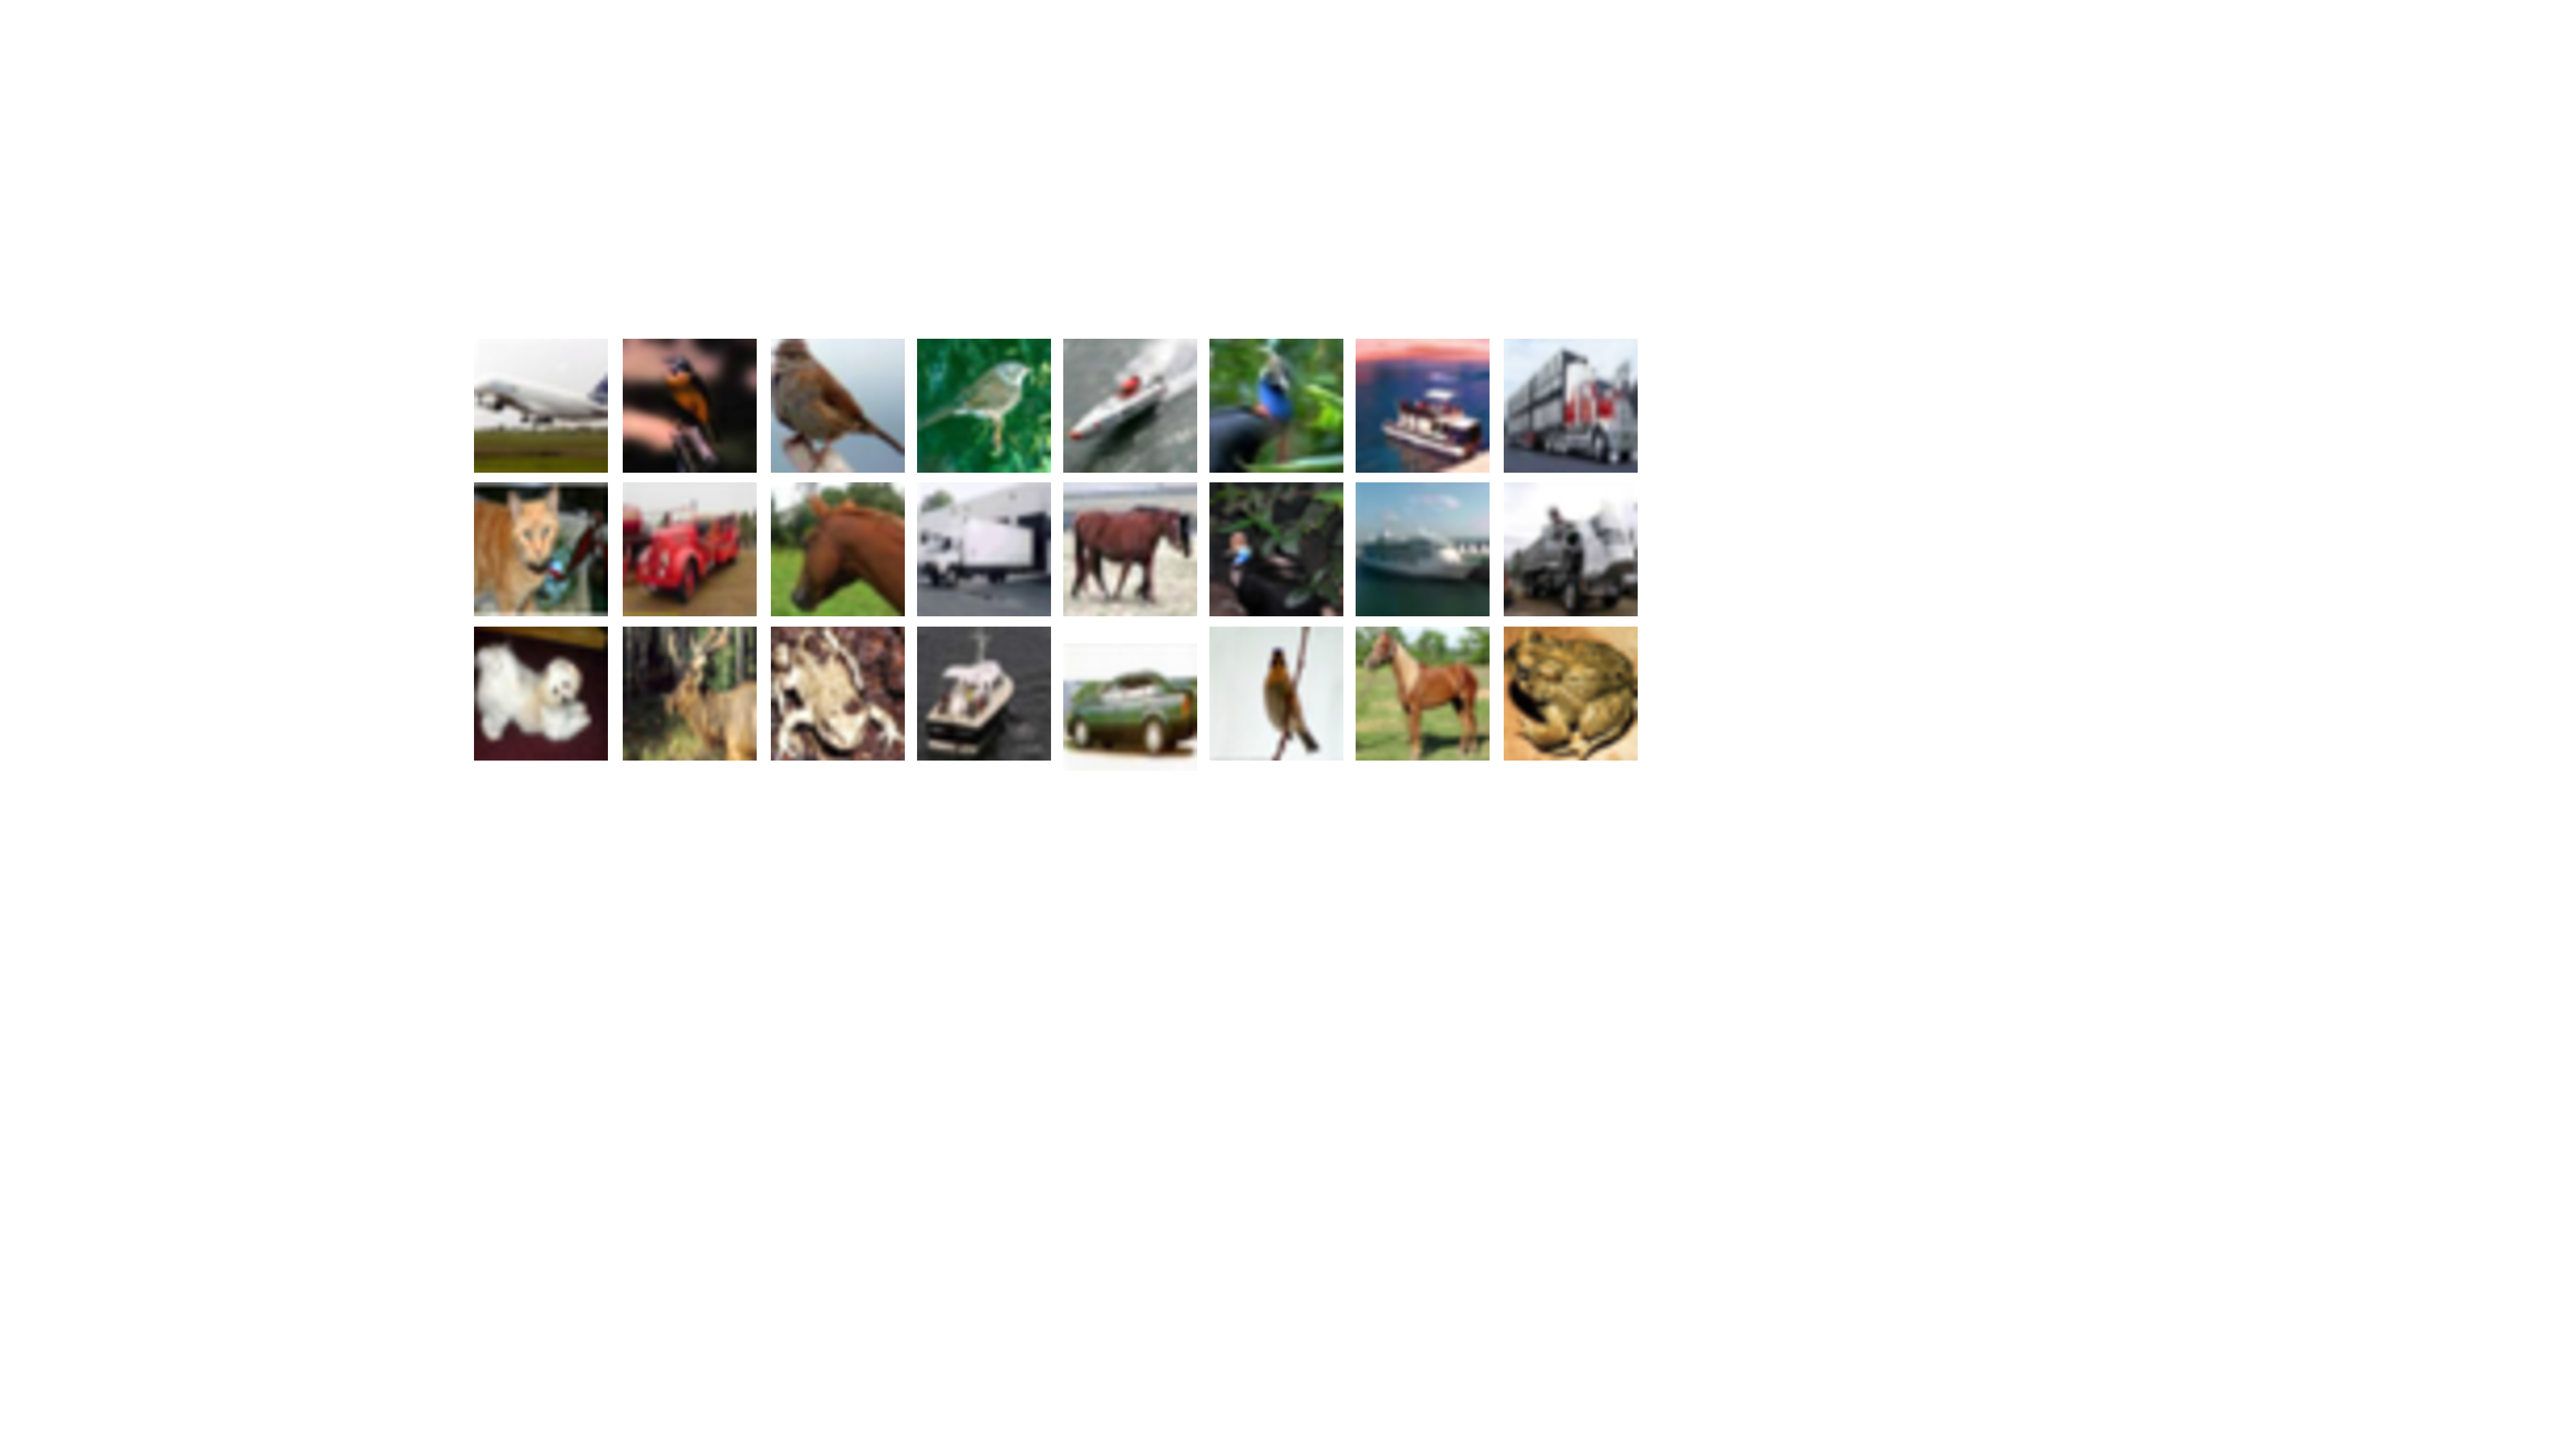
\includegraphics[width=0.9\linewidth]{./figure/entropy_high.pdf}
   \caption{Images of DSV candidates (Selected in the CIFAR-10 dataset).}
   \label{fig:entropyhigh}
\end{figure}
% % \section{DSVs synthethis}
% \begin{figure}[h]
%   \centering
%    \includegraphics[width=0.9\linewidth]{./figure/dsv_all.pdf}
%    \caption{Images of various DSVs  (Synthesized) -- Cat, Ship, Dog, Car, Truck, Bird, Horse, Deer, Plane, Frog.}
%    \label{fig:dsvall}
% \end{figure}
% \section{DSVs synthethis on other architecture}
% \begin{figure}[h]
%   \centering
%    \includegraphics[width=0.9\linewidth]{./figure/diff_architecture.pdf}
%    \caption{Synthesized images on other architecture.}
%    \label{fig:diffarch}
% \end{figure}

\begin{figure}[h]
  \centering
   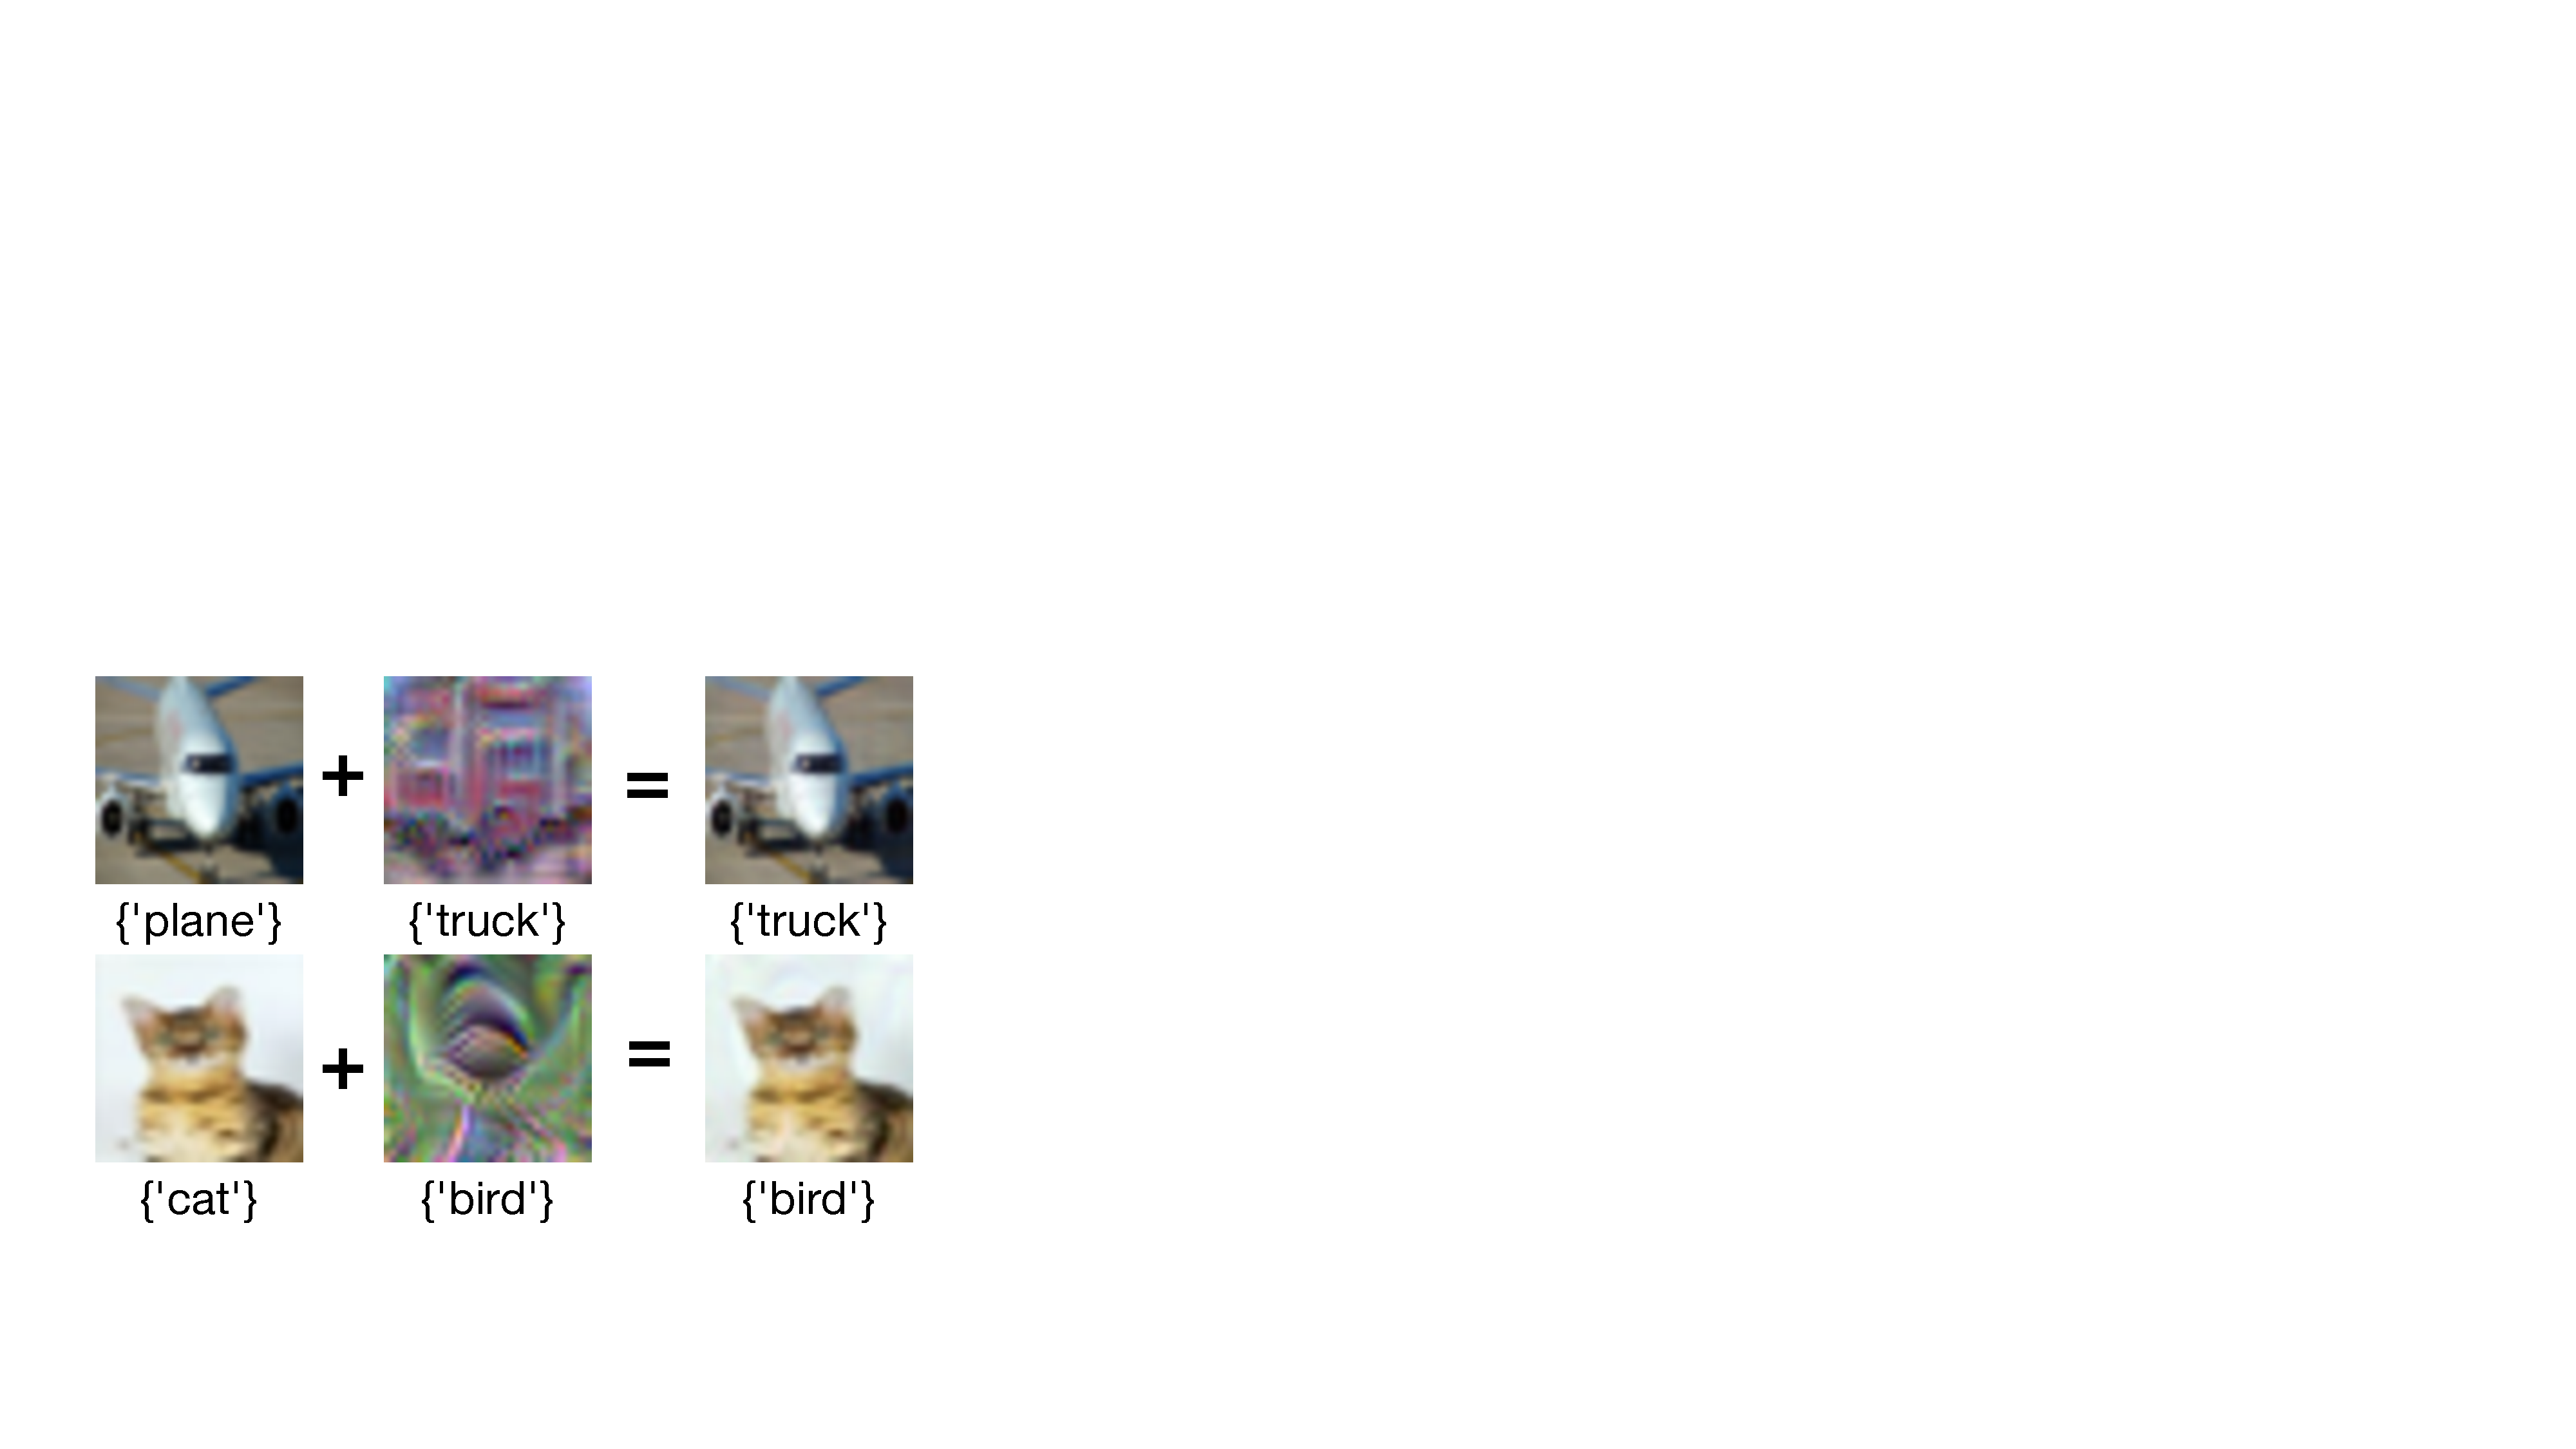
\includegraphics[width=0.5\linewidth]{./figure/adversarial.pdf}
   \caption{\gm{Examples of adversarial attack in the CIFAR-10 dataset}}
   \label{fig:adversarial}
\end{figure}


\begin{figure}[h]
  \centering
   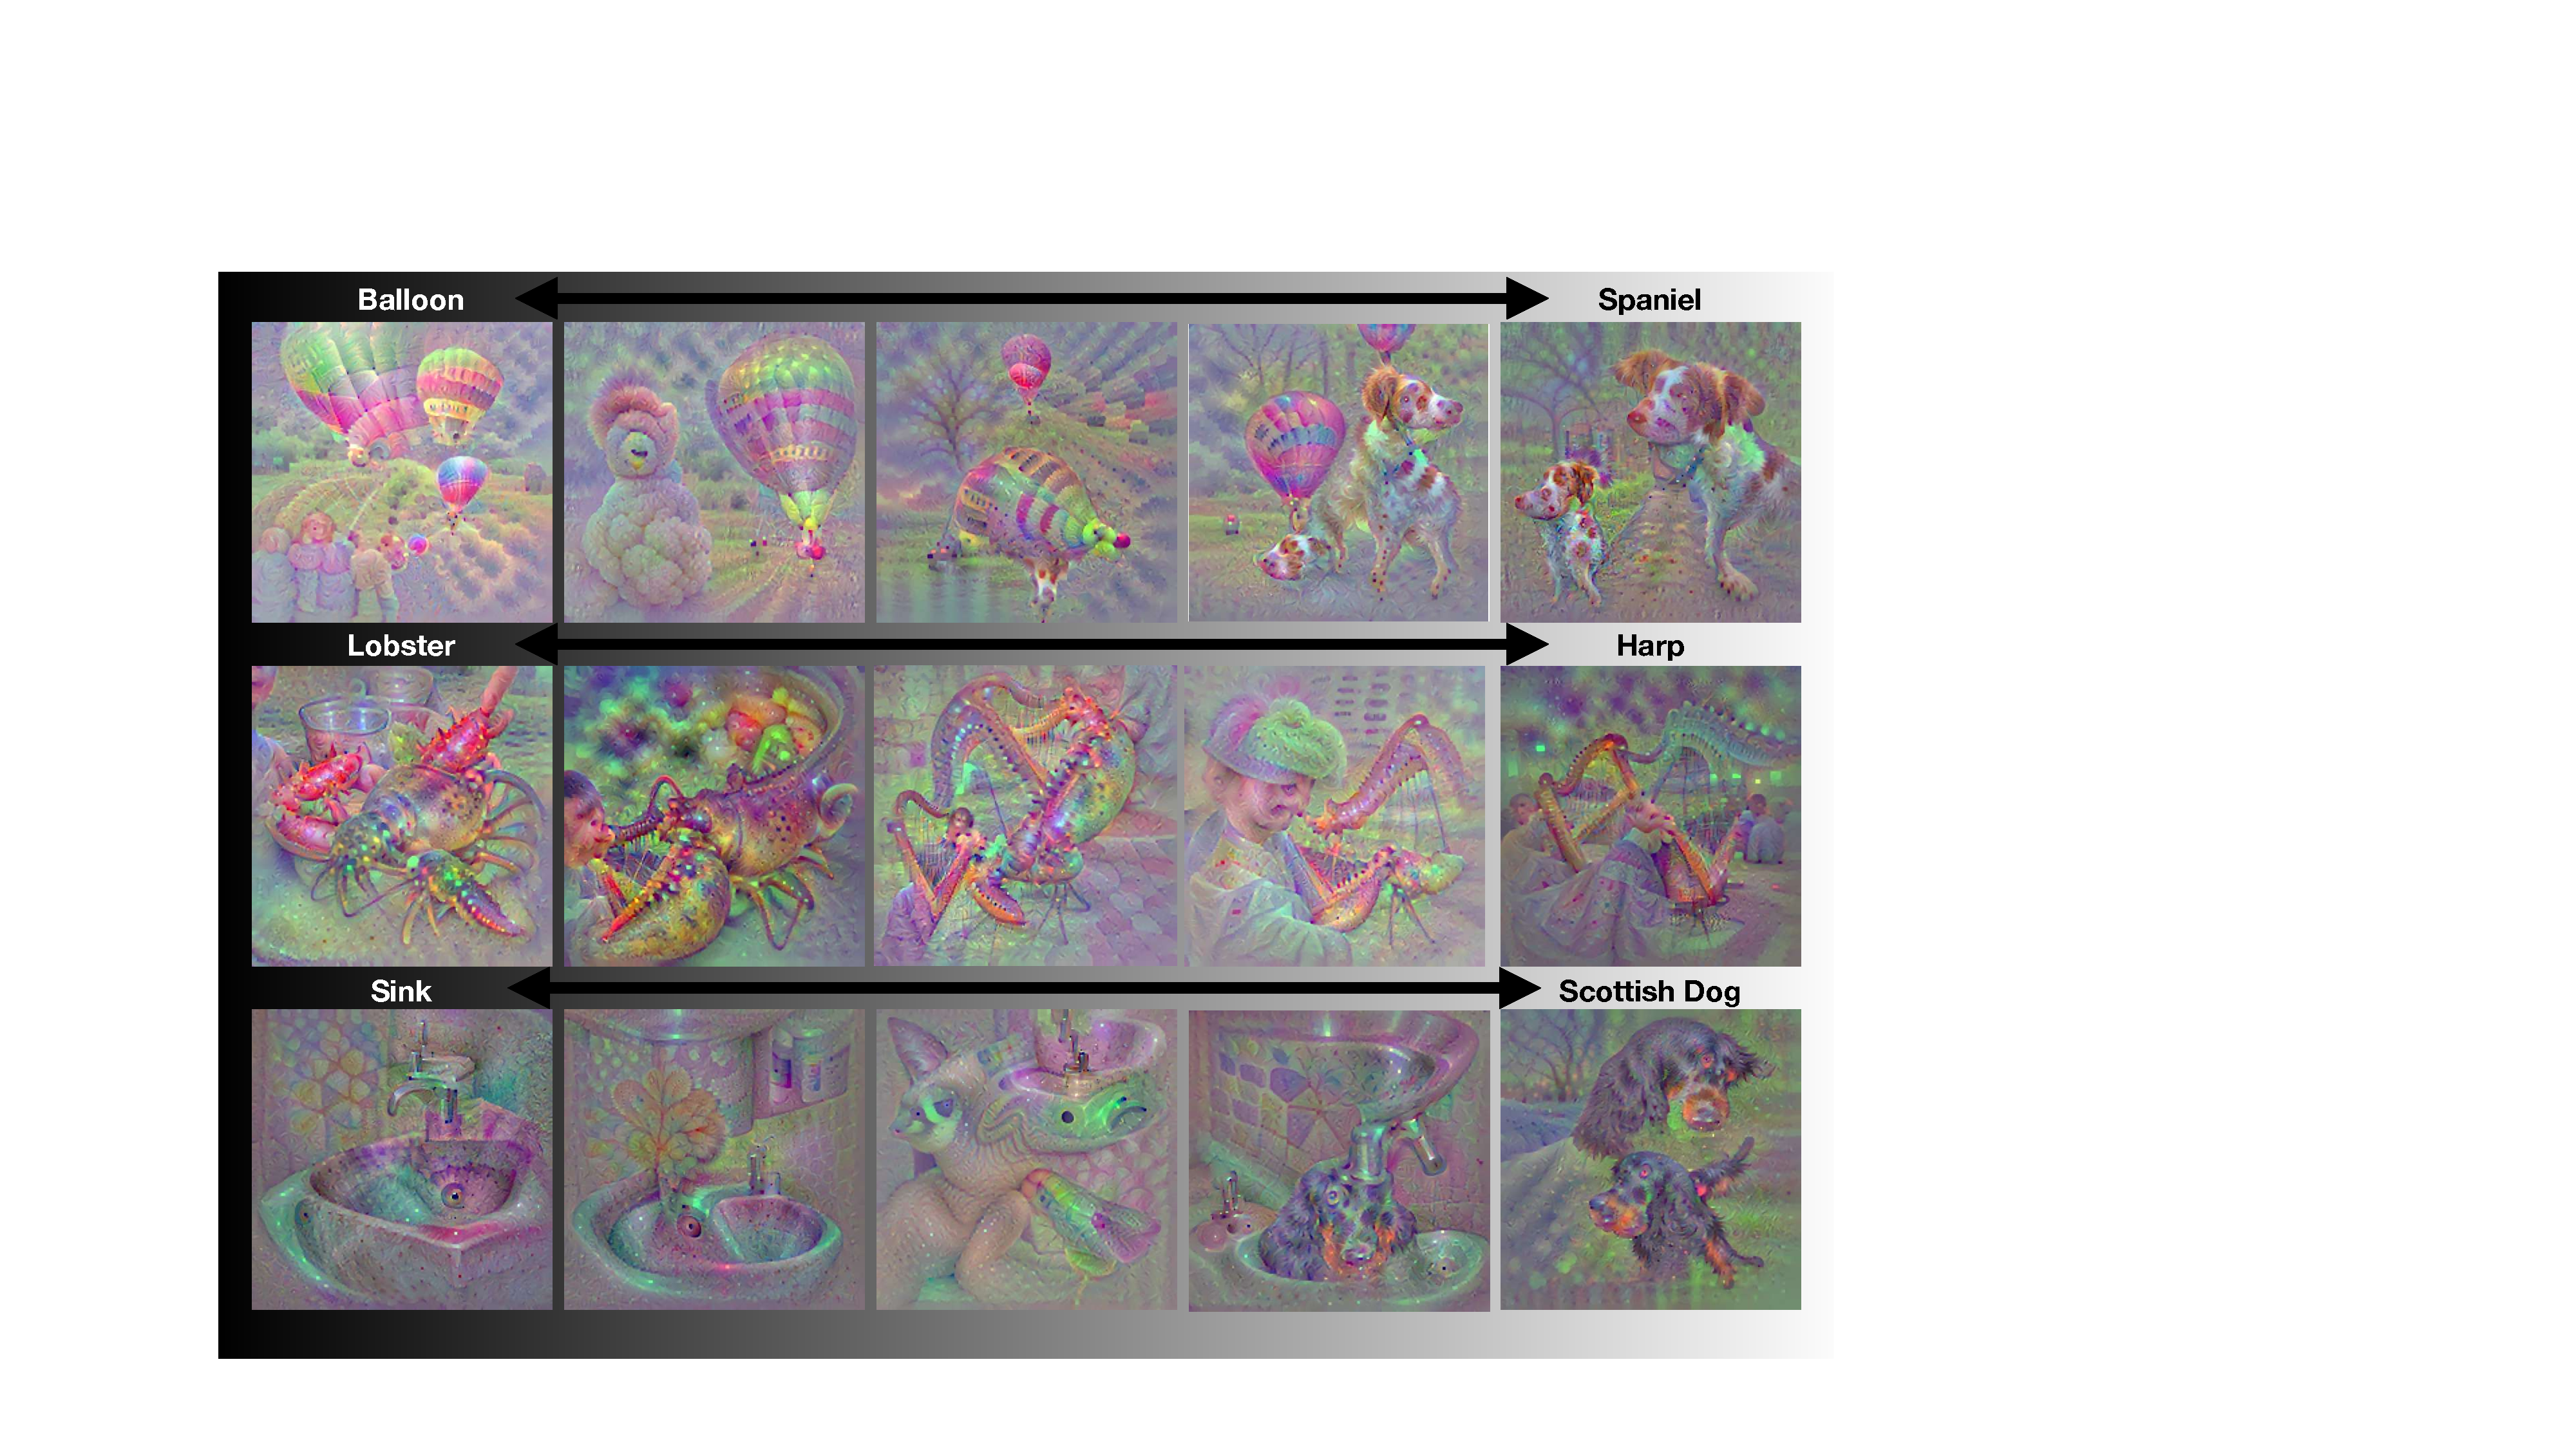
\includegraphics[width=0.9\linewidth]{./figure/mixup_overall.pdf_compressed.pdf}
   \caption{More examples of latent interpolation in the ImageNet dataset}
   \label{fig:latentmore}
\end{figure}



\begin{figure}[h]
  \centering
   \includegraphics[width=0.9\linewidth]{./figure/dsv_cifar100.png}
   \caption{\gm{More examples of generated images with CIFAR-100 dataset}}
   \label{fig:dsv_cifar100}
\end{figure}

\begin{figure}[h]
  \centering
   \includegraphics[width=0.9\linewidth]{./figure/dsv_imagenet.png}
   \caption{More examples of generated images with ImageNet dataset}
   \label{fig:dsv_imagenet}
\end{figure}

\begin{figure}[h]
  \centering
   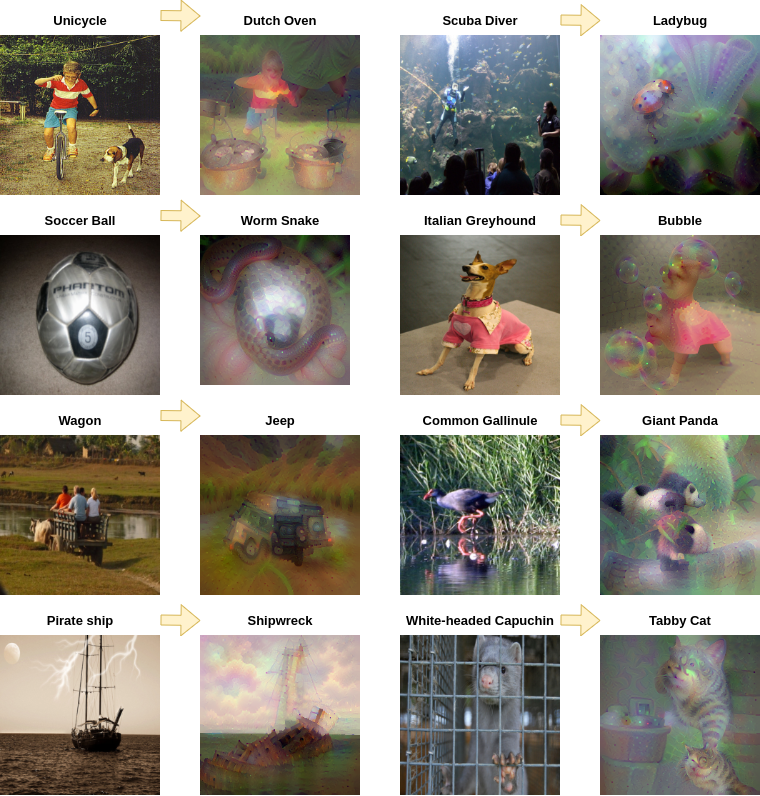
\includegraphics[width=0.9\linewidth]{./figure/editing.png}
   \caption{\gm{More examples of image editing. The images to the left of the arrows represent the initial images before training, while those to the right depict the edited images after training.}}
   \label{fig:dsv_editing}
\end{figure}

\begin{figure}[h]
  \centering
   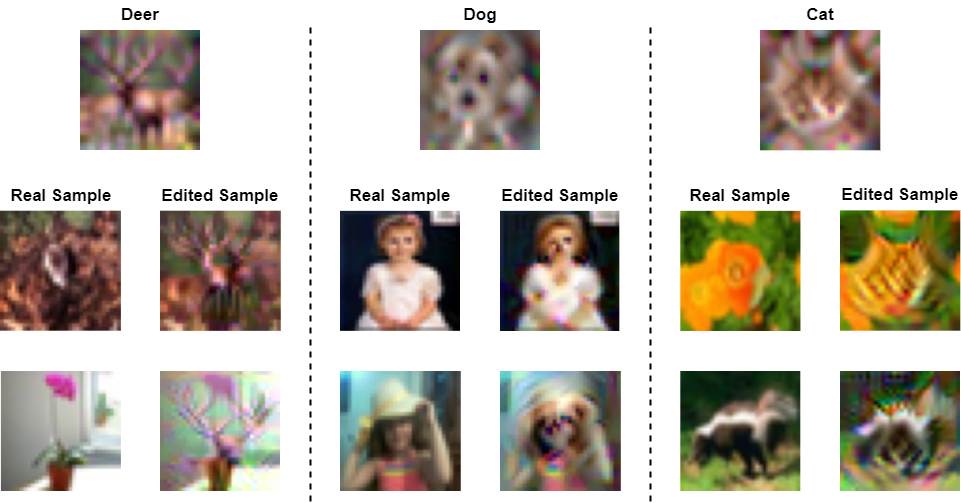
\includegraphics[width=0.9\linewidth]{./figure/decision_criterion.png}
   \caption{\gm{More examples of image editing. The images to the left of the arrows represent the initial images before training, while those to the right depict the edited images after training.}}
   \label{fig:decision_criterion}
\end{figure}

\section{More Characteristics of DSVs}
\paragraph{DSVs Are Full of Discriminative Information}

\jh{In Fig.~\ref{fig:adversarial}, we conducted an experiment by mixing a randomly sampled image from the real dataset with an image from the DSVs. %The norm of the DSV image is about 1\% of that of a real dataset image. 
Upon observation, the mixed image is virtually indistinguishable from an image obtained solely from the real dataset.}
\jh{It is noteworthy to highlight this situation resembles that of an adversarial attack \citep{xu2019adversarial, adversaraialuniversal}, yet we did not apply gradient descent to the image; we simply mixed two images. This suggests that the \nj{discriminative} informational density in a single DSV image is substantially greater than that in a randomly sampled image. The fact that the DSV's characteristics remained dominant in the classification, %despite the greater emphasis on the random image, 
underscores the significant role of DSVs in explaining the model's classification ability.}



% \jh{Fig.~\ref{fig:more_explanation} empirically supports on our assertion on decision criterion. Starting from CIFAR100 random images and CIFAR10-pretrained models, we edited the image cifar10 labels as latents. The edited images changes the image following decision criterions in generated DSVs. 1) For editing images to deer, antler grows. 2) For dog editing, facial dots are generated. 3) For cat editing, pointed traiangler features are generated.}

% \paragraph{DSVs Are Full of Discriminative Information}

% \jh{In Fig.~\ref{fig:adversarial}, we conducted an experiment by mixing a randomly sampled image from the real dataset with an image from the DSVs. %The norm of the DSV image is about 1\% of that of a real dataset image. 
% Upon observation, the mixed image is virtually indistinguishable from an image obtained solely from the real dataset.}
% \jh{It is noteworthy to highlight this situation resembles that of an adversarial attack \citep{xu2019adversarial, adversaraialuniversal}, yet we did not apply gradient descent to the image; we simply mixed two images. This suggests that the \nj{discriminative} informational density in a single DSV image is substantially greater than that in a randomly sampled image. The fact that the DSV's characteristics remained dominant in the classification, %despite the greater emphasis on the random image, 
% underscores the significant role of DSVs in explaining the model's classification ability.}
% \begin{algorithm}[tb]
%    \caption{Support Vector Refinement for Deep Learning Model}
%    \label{alg:KKT}
% \begin{algorithmic}
%    \STATE {\bfseries Input:} Pretrained model $\Phi(\cdot; \theta)$, loss function $L$, augmentation function set $A$, number of DSV candidate $N$, number of class $C$, hyperparameter $\beta$, $\gamma$, \jh{$\alpha_\lambda$, $\alpha_x$}
%    \STATE {\bfseries Ensure:} Freeze model $\Phi(\cdot; \theta)$
%    \STATE Initialize $N \times C$ number of support vector candidates
%    \FOR{$c=1$ {\bfseries to} $C$}
%    \STATE Sample $N$ number of ($x^c_i$,$\lambda^c_i$) for label $c$
%    \ENDFOR
%    \STATE Define  $X = \{ x^c_i \mid c \in [C] , i \in [N]\} $
%    \STATE Define  $\Lambda = \{ \lambda^c_i \mid c \in [C] , i \in [N]\} $
%    \REPEAT
%    \STATE $L_{\text{primal}}(X) = (\sum_{i=1}^{N}\sum_{c=1}^{C} L(\Phi(x^c_i;\theta), c))/NC$
%    \STATE$L_{\text{stat}}(X) = ||\theta + \sum_{i=1}^{N}\sum_{c=1}^{C} \lambda^c_i \nabla_\theta L(\Phi(x^c_i;\theta), c)||^2_2$
%    \STATE $L_{\text{kkt}}(X) = L_{\text{primal}}(X) + \beta \times L_{\text{stat}}(X)$
%    \STATE Sample $f_A \in A$
%    \STATE Define $X' = \{ f_A(x^c_i) \mid x^c_i \in X\} $
%    %\STATE \nj{${L_{akkt}(X)} = {L_{kkt}(X')}$ }
%    \STATE ${L_{total}(X)} = {L_{kkt}(X)} + \gamma \times {L_{kkt}(X')}$
%    \STATE Update $x_i^c \leftarrow x_i^c - \jh{\alpha_x}\nabla_{x_i^c} L_{total}(X)$, \quad  $\forall \  i \ \text{and} \ c$
%    \STATE Update $\lambda_i^c \leftarrow \lambda_i^c -\jh{\alpha_\lambda}\nabla_{\lambda_i^c} L_{total}(X)$, \quad  $\forall \  i \ \text{and} \ c$
%    \STATE Remove $x^c_i$ from $X$ if corresponding $\lambda^c_i < 0$
%    \UNTIL{$X$ converges}
%    \STATE {\bfseries Return:} Set of DSV : $X$
% \end{algorithmic}
% \end{algorithm}

\section{More Examples}
\jh{In Fig.~\ref{fig:latentmore}, examples of latent interpolations between target labels are presented. The smoothness of these interpolations within the latent space indicates that the semantic information learned from the training data has been effectively applied during the DSV generation process. This observation provides evidence that the DeepKKT optimization successfully conducts the generative process.}

\gm{Fig.~\ref{fig:dsv_cifar100} and ~\ref{fig:dsv_imagenet} provide examples of deep support vectors generated using the CIFAR-100 and ImageNet datasets, respectively. Fig.~\ref{fig:dsv_editing} presents additional examples related to image editing.}

% \jh{Fig.~\ref{fig:more_explanation} empirically supports on our assertion on decision criterion. Starting from CIFAR100 random images and CIFAR10-pretrained models, we edited the image cifar10 labels as latents. The edited images changes the image following decision criterions in generated DSVs. 1) For editing images to deer, antler grows. 2) For dog editing, facial dots are generated. 3) For cat editing, pointed traiangler features are generated.}

\jh{Fig.~\ref{fig:decision_criterion} empirically supports on our assertion on decision criterion. Starting from CIFAR100 random images and CIFAR10-pretrained models, we edited the image \hh{CIFAR10} labels as latents. The edited images changes the image following decision criterions in generated DSVs. 1) For editing images to deer, antler grows. 2) For dog editing, facial dots are generated. 3) For cat editing, pointed traiangler features are generated.}



\section{Algorithm}
\label{sec:alg}
Alg.~\ref{alg:KKT} presents our algorithm of generating Deep Support Vectors (DSVs).
Initialized either from a noise $x_i^s \sim \mathcal{N}(0,I)$ or a real sample, it iterates to obtain the primal $X^S$ and dual $\Lambda^S$ variables.  

\begin{algorithm*}[h]
\caption{Support Vector Refinement for Deep Learning Model }\label{alg:KKT}
\begin{algorithmic}[1]
\Require Pretrained classifier $\Phi(\cdot; \theta)$, loss function $L$, augmentation function set $A$, number of DSV candidate $N$, number of class  $C$, hyperparameters $\alpha$, $\beta$
\Ensure Freeze classifier $\Phi(\cdot; \theta)$

\State Initialize $N \times C$ number of support vector candidates
\For{$i = 1$ to $C$}
    \State sample $N$ number of $(x^s_i, \lambda^s_i)$ for label $y^s_i = i$
\EndFor
\State Define $X^S = \{ x^s_i \mid i \in [C], s \in [N]\}$
\State Define $\Lambda^S = \{ \lambda^s_i \mid i \in [C], s \in [N]\}$
\Repeat
    \State $L_{\text{primal}}(X^S) = \sum_{s=1}^{N} \sum_{i=1}^{C} L(\Phi(x^s_i;\theta), y^s_i)$
    \State $L_{\text{stationary}}(X^S) = \|\theta + \sum_{s=1}^{N} \sum_{i=1}^{C} \lambda^s_i y^s_i \nabla_\theta \Phi(x^s_i;\theta)\|^2_2$
    \State $L_{\text{kkt}}(X^S) = \beta_1 \cdot L_{\text{primal}}(X^S) +  L_{\text{stationary}}(X^S)$
    \State $L_{\text{prior}}$ = $\beta_2 \cdot L_{\text{tot}}(X) + \beta_3 L_{\text{norm}}(X)$
    \State Sample $f_A \in A$
    \State Define $AX^S = \{ f_A(x^s_i) \mid x^s_i \in X^S\}$
    \State $L_{\text{akkt}}(X^S) = L_{\text{kkt}}(AX^S)$  
    % \State $L_{\text{total}}(X^S) = L_{\text{kkt}}(X^S) + \beta \cdot L_{\text{akkt}}(X^S)$ + \jh{L_{\text{prior}}}
    \State $L_{\text{total}}(X^S) = L_{\text{kkt}}(X^S) + \eta \cdot L_{\text{akkt}}(X^S)$ + \jh{$L_{\text{prior}}$}
    \State Update $X^S \leftarrow X^S + \nabla_{X^S} L_{\text{total}}(X^S)$
    \State Update $\Lambda^S \leftarrow \Lambda^S + \nabla_{\Lambda^S} L_{\text{total}}(X^S)$
    \State Remove $x^s_i$s for corresponding $\lambda^s_i < 0$
\Until{$X^S$ converges}
\State \Return Set of DSV : $X^S$
\end{algorithmic}
\end{algorithm*}





% \begin{algorithm*}[h]\label{alg:KKT}
% \caption{Support Vector Refinement for Deep Learning Model}
% \begin{algorithmic}[1] 
% \Require Pretrained classifier $\Phi(\cdot; \theta)$, loss function $L$, augmentation function set $A$, number of DSV candidate $N$, number of class  $C$, hyperparmeter $\alpha$, $\beta$
% \Ensure Freeze classifier $\Phi(\cdot; \theta)$
% \State Initialize $N$*$C$ number of support vector candidates
% \For{i=1 to $C$}
% \State sample $N$ number of ($x^s_i$,$\lambda^s_i$) for label $y^s_i = i$
% \EndFor
% \State Define  $X^S = \{ x^s_i \mid i \in [C] , s \in [N]\} $
% \State Define  $\Lambda^S = \{ \lambda^s_i \mid i \in [C] , s \in [N]\} $
% \Repeat
%     \State $L_{\text{primal}}(X^S) = \sum_{s=1}^{N}\sum_{i=1}^{C} L(\Phi(x^s_i;\theta^*), y^s_i)$
%     \State $L_{\text{stationary}}(X^S) = ||\theta^* + \sum_{s=1}^{N}\sum_{i=1}^{C} \lambda^s_i y^s_i\nabla_\theta\Phi(x^s_i;\theta^*)||^2_2$
%     \State $L_{\text{kkt}}(X^S) = L_{\text{primal}}(X^S) + \alpha * L_{\text{stationary}}(X^S)$
%     \State Sample $f_A \in A$
%     \State Define $AX^S = \{ f_A(x^s_i) \mid x^s_i \in X^S\} $
%     \State ${L_{akkt}(X^S)} = {L_{kkt}(AX^S)}$ 
%     \State ${L_{total}(X^S)} = {L_{kkt}(X^S)} + \beta * {L_{akkt}(X^S)}$
%     \State Update $X^S \longleftarrow X^S + \nabla_{X^S} L_{total}(X^S) $
%     \State Update $\Lambda^S \longleftarrow \Lambda^S + \nabla_{\Lambda^S} L_{total}(X^S) $
%     \State Remove $x^s_i$s for corresponding $\lambda^s_i < 0$
% \Until{$X^S$ converges}
% \State \Return Set of DSV : $X^S$
% \end{algorithmic}
% \end{algorithm*}